\documentclass{article}
\usepackage[margin=1in]{geometry}
\usepackage[affil-it]{authblk}


%
%This is a LaTeX document for organizing the Related Work on the 3-D Printed UAS project
%
% To compile this into a .pdf simply run 'pdflatex 3DUAS_RelatedWork.tex' on the command line.
% To automatically generate the bibliography, then run 'bibtex 3DUAS_RelatedWork' and then repeat the command 'pdflatex 3DUAS_RelatedWork.tex' twice.
%

\usepackage{amsmath}
%\usepackage{times}
%\usepackage{mathtime} 
\usepackage{pslatex} %regular times font/smaller courier font
\usepackage{amssymb}
\usepackage{alltt}
\usepackage{longtable}
\usepackage{multirow}
\usepackage{url}
\usepackage{mathrsfs} %for \mathscr{} 
\usepackage{multicol}
\usepackage{capt-of}
\usepackage[toc,page]{appendix}
\usepackage{booktabs}
\usepackage{listings}
\usepackage{color}

\lstset{frame=tb,
  aboveskip=3mm,
  belowskip=3mm,
  showstringspaces=false,
  columns=flexible,
  basicstyle={\small\ttfamily},
  numbers=none,
  numberstyle=\tiny\color{gray},
  keywordstyle=\color{blue},
  commentstyle=\color{dkgreen},
  stringstyle=\color{mauve},
  breaklines=true,
  breakatwhitespace=true,
  tabsize=3
}

%\newtheorem{thm}{Theorem}[section]
\newtheorem{cor}{Corollary}
\newtheorem{lem}{Lemma}
\newtheorem{defin}{Definition}
%Use like this: \begin{lem}\label{...}  .... \end{lem}

%%%%%%%%%%%%%%%%%%%%%%%%%%%%%%%%%%%%%%%%%%%%%%%%%%%%%%%%
% Figure Magic
%%%%%%%%%%%%%%%%%%%%%%%%%%%%%%%%%%%%%%%%%%%%%%%%%%%%%%%%
\usepackage{gastex} % pictures on steroids
\usepackage{epsfig}
\usepackage{float}
\usepackage{graphicx}
\usepackage{caption}
\usepackage{subcaption}
\renewcommand{\topfraction}{.95} %figures can take up at most 95% of the page before being alone
\renewcommand{\bottomfraction}{.99} %figures can take up at most 99% of the page before being alone
\renewcommand{\textfraction}{.1} %at most this this % of page will be text before making figure-only page

%%%%%%%%%%%
% Block Quotes       %
%%%%%%%%%%%
\newenvironment{blockquote}{
  \par
  \medskip
  \leftskip=4em\rightskip=2em
  \noindent\ignorespaces}{
  \par\medskip}

%for code listings
%\usepackage{listings}
%\usepackage{courier}




\begin{document}




\section{Jessica Glass - Week 2 Update}

\subsection{Airspace Classes and Defining Terminal Procedures}

\subsubsection*{Flight Modes in VFR}

\begin{figure}[H]
\centering
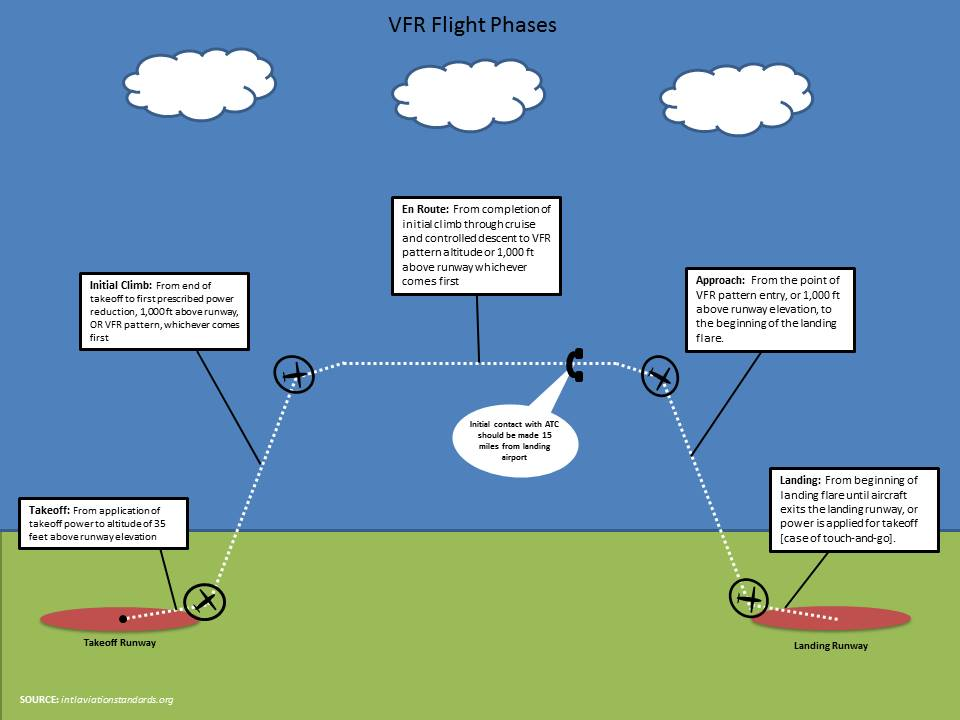
\includegraphics[scale=0.5]{VFR_flight_phases.jpg} 
\end{figure}

\subsubsection*{Airspace Classes}

\begin{itemize}
\item {\bf Class A} extends from 18,000' to 60,000' MSL
\item {\bf Class B} [In general, 10,000' surrounding nation's busiest airports] The MSL ceiling 
and floor altitudes of each sector are shown with last two zeros emitted on TAC
\item {\bf Class C} Generally from surface to 4,000 feet above above airport elevation surrounding
airports that have an operational control tower, serviced by radar approach control, and
have certain number of IFR operations/passenger enplanements.  surface area of 5 NM, an outer
circle with a 10 NM radius that extends 1200 ft to 4000 ft above airport elecation
\item {\bf Class D} Generally from surface to 2,500 ft above airport with operating control tower
\item {\bf Class E} Everything in between [below class A, space in between airports]

\end{itemize}

\subsubsection*{VFR Entry and Weather Requirements in Terminal Airspace Classes (B,C,D)}

\begin{figure}[H]
\centering
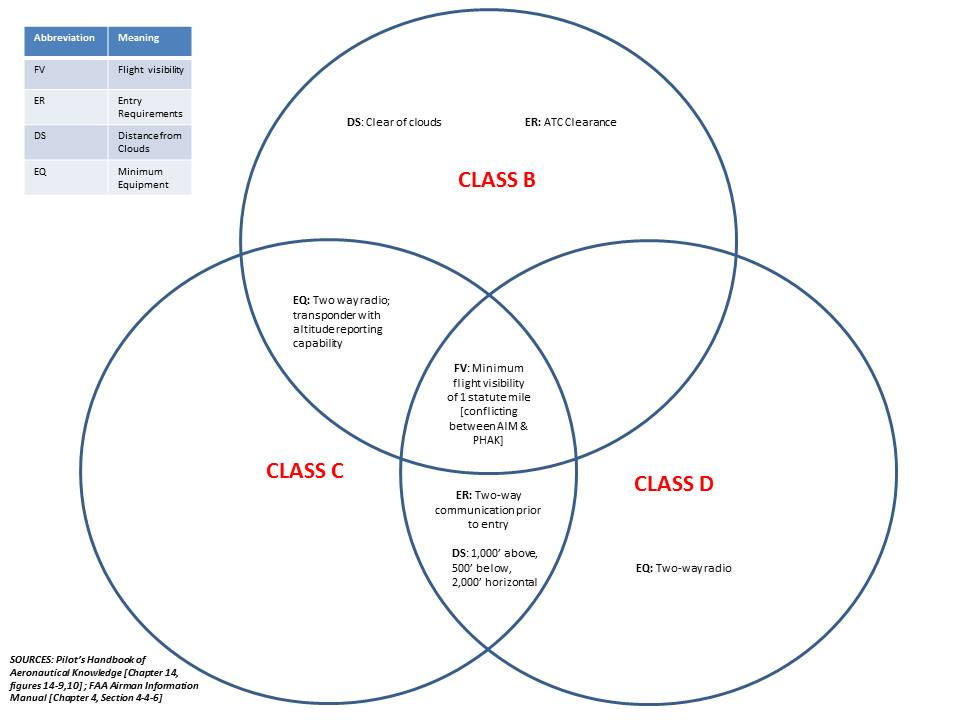
\includegraphics[scale=0.5]{VFR_Weather_minimums.jpg} 
\end{figure}

\subsection{Traffic Patterns}


\subsubsection*{Airport Traffic Patterns [General Case]}


\begin{figure}[H]
\centering
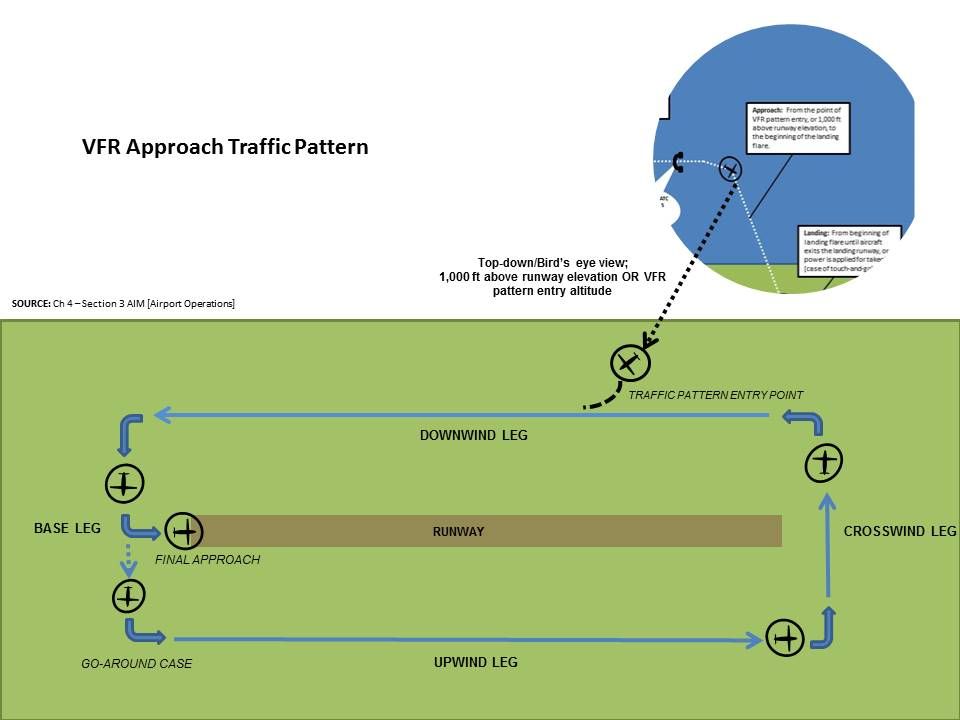
\includegraphics[scale=0.5]{final_approach_traffic_pattern.jpg} 
\end{figure}


\begin{itemize}
\item All turns made left, unless specified to the right by visual lighting patterns
\item Standard, rectangular traffic pattern is typically executed at an altitude of 1,000 ft above airport elevation
\item Operate at a speed of no more than 200 knots
\item When approaching airport, traffic pattern should be entered at a 45 degree angle to the downwind leg
\end{itemize}

\subsubsection*{Traffic Patterns [Downwind leg]}

\begin{itemize}
\item Landing gear extended
\item Altitude maintained until abeam end of the approach runway
\item Once reaching abeam runway, power should be reduced and descent begins
\item Downwind leg continues to a point approximately 45 degrees from approach end of runway
\end{itemize}

\subsubsection*{Traffic Patterns [Base leg]}

\begin{itemize}
\item Perpendicular to centerline of landing runway
\item Established as a sufficient distance from approach end of runway to permit gradual descent
\end{itemize}

\subsubsection*{Traffic Patterns [Final Approach]}

\begin{itemize}
\item When two or more aircraft approach, aircraft with lower altitude have right-of-way
\end{itemize}

\subsubsection*{Traffic Patterns [Upwind Leg]}

\begin{itemize}
\item Transitional part of traffic pattern when on final approach, a go-around is initiated and climb altitude established
\item When safe altitude is attained, pilot commences shallow bank to crosswind side
\end{itemize}

\subsubsection*{Traffic Patterns [Departure Leg]}

\begin{itemize}
\item Straight course leading from take-off runway
\item Begins at point from airplane leaving the ground to entrance into traffic pattern
\item When departing, ATC will give aircraft one of the following instructions:
\begin{itemize}
\item Continue straight
\item 45 degree left hand turn (in the case of left turn traffic pattern), vice versa for right hand turn traffic patterns
\item Turn 90 degrees into traffic pattern crosswind leg
\end{itemize}
\end{itemize}

\subsection{Approaches and Landings}

\subsubsection*{Base Leg Normal Approach}
\begin{itemize}
\item Landing gear should already be extended
\item After turning onto base leg, pilot should descend with reduced power and airspeed of 1.4$V_{SO}$
\item Ensure turn to final approach is gradual and not too steep causing high stall conditions
\item Ensure plane is angled such that the crosswind won't cause it to drift too far from landing runway
\end{itemize}

\subsubsection*{Final Approach}
\begin{itemize}
\item Allign with centerline of runway
\item Flaps put into landing position and pitch attitude adjusted for desired rate of descent 
\end{itemize}

\subsection{ATC Clearances and Aircraft Separation}

\subsubsection*{General}
\begin{itemize}
\item Clearance limit - ATC will authorize airport of intending landing prior to departure
\item Departure procedure - headings to fly and altitude restrictions may be issued to separate a departure from other traffic
\item If no holding instructions have been issued, pilot should ask ATC for holding instructions
\item When aircraft is 3 minutes or less from clearance limit and clearance beyond fix not received, pilot is expected to start speed reduction
\item Pilot should report when reaching clearance limit
\end{itemize}

\subsubsection*{VFR Clearances}

\begin{itemize}
\item ATC clearance prior to entry
\item Clear of clouds
\item 1 mile visibility
\item 1 statute mile ground visibility for taking off and landing
\item May require flying at or below specific altitude
\item VFR prohibited at night
\item Read back altitudes, altitude restrictions and vectors in the same sequence received
\end{itemize}

\subsection{Decision Chain outline}

To be turned into a diagram for better visual aid.  General outline of sequence of events when finishing en route phase of flight and entering into approach (FOR VFR, NORMAL LANDING)

\begin{itemize}
\item 15 miles from landing airport?
\item Contact ATC - gain clearance for entering airspace
\item Visibility and weather check
\item Enter airspace traffic pattern at 45 degree angle of downwind leg
\item Left turn to base leg
\item Left turn to final approach
\item Land
\item Exit Runway
\item Taxi to final destination

\end{itemize}

\subsection{Questions and Comments}

\begin{itemize}
\item This past week also involved working through plexil workshops and better understanding how the plexil plans are executed and simulated
\item I think that I am at a point where I understand the terminal procedures very well at a high level and am ready to begin purely working in plexil on week 3.  
\item Terminal procedures rely heavily on dialogue between pilot and ATC, a capability which isn't currently supported for AOS plexil.  Is there a way to simulate/go around this for the time being?  If so, what is the best way to go about this
 
\end{itemize}


\end{document}